\chapter{Metodologia}
\section{Gerenciamento}

\subsection{Estrutura Analítica do Projeto (EAP)}

A visão geral do sistema pode ser vista na estrutura analítica do projeto abaixo em uma organização das entregas a serem feitas em um formato de árvore, partindo de tarefas mais gerais para tarefas mais específicas. A EAP está estruturada com os entregáveis de cada engenharia no decorrer do projeto. Projeto este foi dividido em quatro frentes com diferentes responsabilidades. Software, responsável pelo aplicativo que liga o cliente ao vendedor, eletrônica responsável pela segurança, sensoriamento e interface humano máquina, estrutura, composta por duas engenharias, automotiva e aeroespacial e por fim alimentação, composta sob responsabilidade da engenharia de energia.  

\begin{figure}[H]
	\centering
    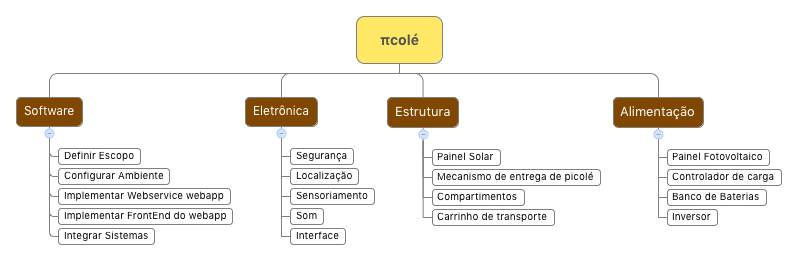
\includegraphics[width=\textwidth]{figuras/EAP_Geral}
    \caption{EAP Geral}
    \label{fig:EAP_Geral}
\end{figure}

\subsection{Alocação dos Recursos Humanos}
A metodologia utilizada para o gerenciamento da equipe é o Scrum com algumas adaptações. Este \textit{framework} é ideal para o desenvolvimento de projetos complexos, no qual produtividade e criatividade são necessárias para a entrega de produtos de alto valor.

De acordo com \cite{the_scrum_guide} Scrum é baseado em três pilares: transparência dos processos, como as atividades a serem feitas, inspeção dos artefatos para garantir que o produto esteja sendo construído corretamente, e adaptação dos eventos para se adequar à equipe, como \textit{sprint planning}, \textit{daily scrum}, \textit{sprint review}, e \textit{sprint retrospective}.

A equipe foi dividida em quatro áreas, que são área de estrutura, de energia, de eletrônica e de software, como mostra a figura \ref{fig:organograma}.

\begin{figure}[H]
	\centering
    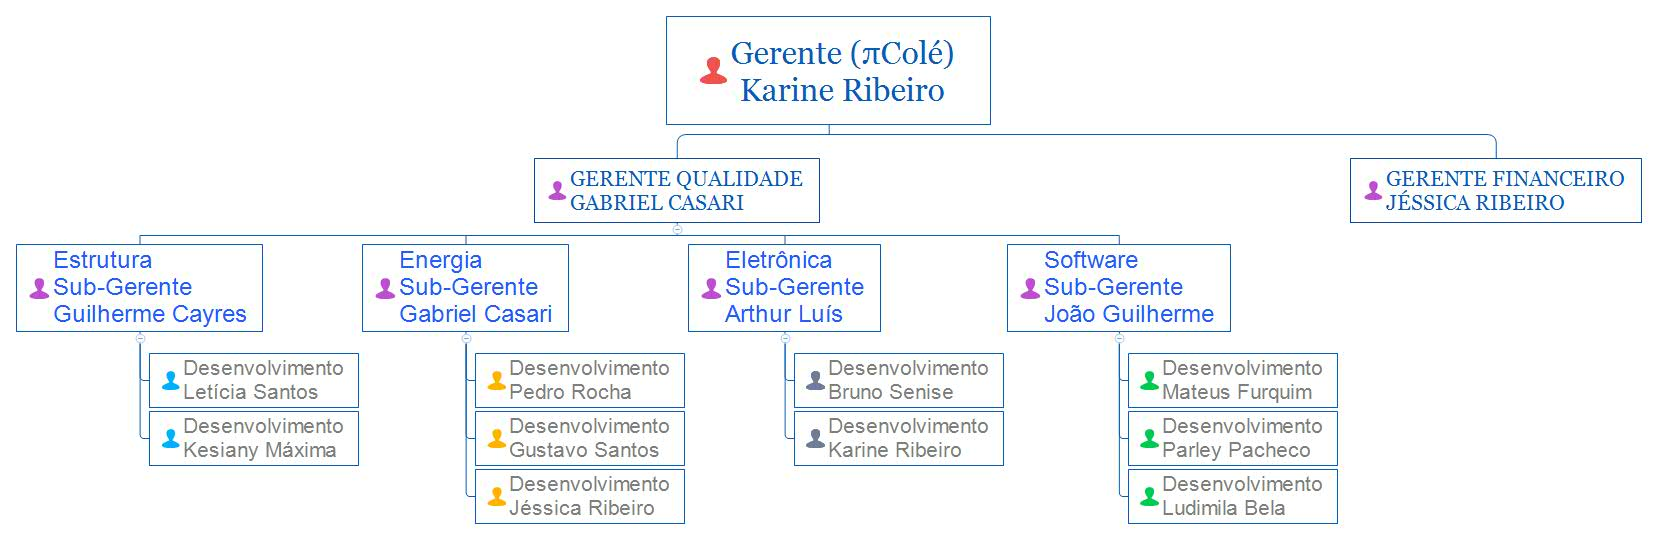
\includegraphics[scale=0.3]{figuras/organograma}
    \caption{Organização Do Projeto}
    \label{fig:organograma}
\end{figure}

A divisão de papéis garante a qualidade do projeto devido às inspeções, que é o segundo pilar do Scrum. O papel de gerente é ser responsável por manter toda a equipe alinhada em relação aos requisitos do projeto e garantir a alta qualidade do produto. Cada área possui um sub-gerente, responsável por reportar, acompanhar e ajudar cada subgrupo. Além disso, existe um gerente financeiro responsável pelo balanço do caixa.

Para cumprirmos com outro pilar do Scrum, terá um quadro para organização de tarefas que estará sempre visível para todos da equipe. Essa transparência das atividades traz consigo confiança e motivação para a equipe.

\begin{figure}[H]
	\centering
    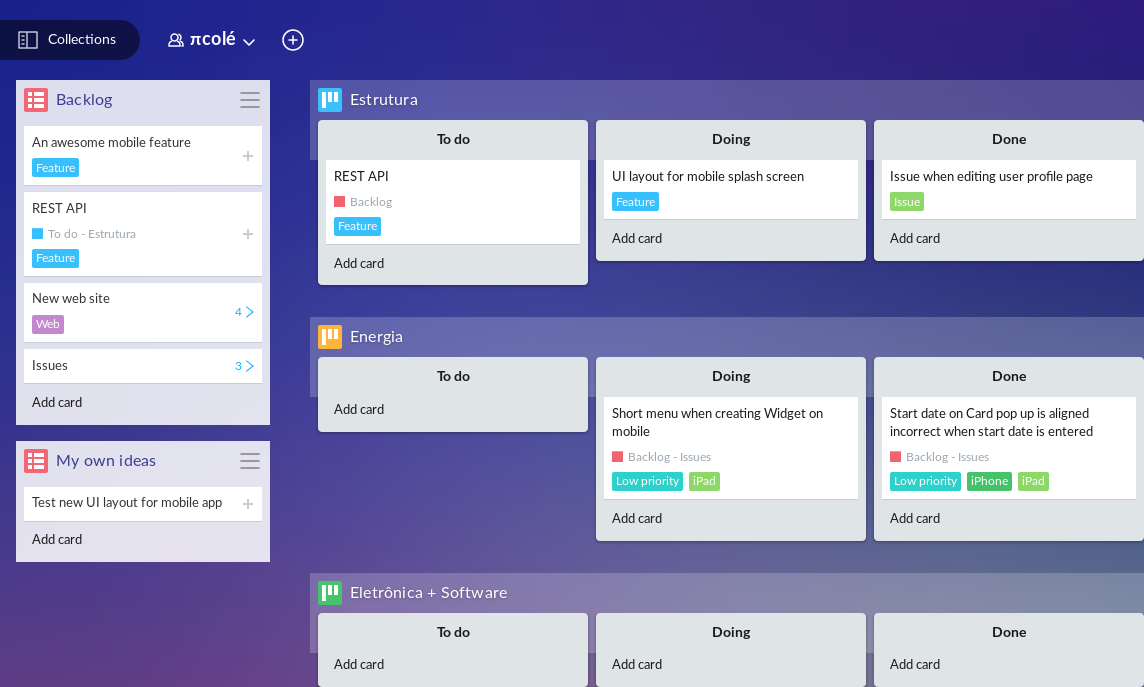
\includegraphics[scale=0.5]{figuras/favro}
    \caption{Tela inicial do favro}
    \label{fig:favro}
\end{figure}

Por fim, o último pilar é a adaptação dos eventos do scrum. O evento adaptado é a reunião diária (\textit{daily meeting}) que passará a ser duas vezes por semana no horário da disciplina. Essa escolha deve-se aos conflitos de horários entre os integrantes. Além disso, caso não haja progresso no projeto em determinado dia, a reunião não se faz necessária.

	O planejamento das sprints será realizado nas sextas-feiras. O objetivo desta reunião é determinar tarefas a serem feitas ao longo da \textit{sprint}. A \textit{sprint} é um período no qual apenas as tarefas definidas no seu planejamento deverão ser feitas. A duração da \textit{sprint} será de 2 semanas e, ao final, será realizado uma revisão. Está reunião ao fim da \textit{sprint} deverá revisar o trabalho feito e o \textit{backlog} deve ser atualizado. As tarefas que não foram concluídas podem continuar a ser realizadas na próxima \textit{sprint}. E a última reunião é a retrospectiva, no qual será discutido e levado em conta as pessoas, os relacionamentos, os processos, e as ferramentas.
    
    As ferramentas a serem utilizadas serão o \textit{Slack} para comunicação, o \textit{Favro} para gerenciamento de tarefas, o \textit{Google Drive} para compartilhar  documentos e o \textit{Overleaf} para edição do relatório final.


\subsection{Comunicação}

O sucesso de todo projeto está diretamente relacionado ao engajamento da equipe, sendo assim, é necessário uma comunicação eficaz entre os membros da equipe. A Tabela \ref{tab:comunicacao} detalha os métodos de comunicação utilizados pela equipe.

\begin{table}[H]
\centering
\caption{Métodos de comunicação.}
\label{tab:comunicacao}
\resizebox{\textwidth}{!}{%
\begin{tabular}{|l|l|l|l|l|}
\hline
\textbf{Objetivo}                       & \textbf{Ferramenta}      & \textbf{Frequência}            & \textbf{Horário}               & \textbf{Local}    \\ \hline
Acompanhamento das atividades  & Favro           & Sob demanda           & N/A                   & N/A     \\ \hline
Avisos rápidos/ Lembretes      & Telegram/Slack & Sob demanda           & N/A                   & N/A   \\  \hline
Decisões técnicas/Planejamento & Presencial      & Duas vezes por semana & Horário da disciplina & FGA  \\  \hline
Desenvolvimento do projeto     & Overleaf        & Sob demanda           & A definir             & A definir
\\ \hline \end{tabular}%
}
\end{table}



\subsection{Tempo}


Para a definição das atividades a serem realizadas durante o projeto utilizou-se como base os pacotes de trabalho estabelecidos na Estrutura Analítica do Projeto (EAP),
onde os mesmos foram devidamente decompostos com base nos três grandes marcos do projeto referentes às entregas de Ponto de Controle 1, 2 e 3. Para tal feito, a equipe precisará cumprir as atividades elucidadas no cronograma.

Após decompostos os pacotes de trabalho da EAP, a equipe de gerência reuniu-se para discutir como suas atividades seriam executadas, visando tanto uma paralelização
de atividades quanto o tempo estimado e os recursos necessários para tal.
Para a determinação do tempo foram utilizadas as técnicas de Analogia e Decisão em Grupo, as quais, segundo o \cite{PMBK}, representam:

\begin{itemize}

\item Analogia: baseia-se em pacotes de trabalho/atividades similares de projetos anteriores para estimar a duração dos pacotes de trabalho e/ou atividades do seu projeto
atual.

\item Decisão em Grupo: nessa técnica o envolvimento da equipe de projeto nas estimativas proporcionam comprometimento da mesma com as atividades a serem realizadas.

\end{itemize}

% \newpage
\subsubsection{Cronograma}
O cronograma referente ao nosso projeto encontra-se na tabela \ref{tab:cronograma} abaixo, contendo seus pacotes de trabalho, atividades e datas. 

% \begin{table}[H]
\footnotesize  % Switch from 12pt to 11pt; otherwise, table won't fit
\setlength\LTleft{-40pt}            % default: \fill
\setlength\LTright{\fill}           % default: \fill
% \resizebox{\textwidth}{%
\begin{longtable}{|c|m{6.5cm}|m{3.2cm}|m{3.2cm}|c|}
% \centering
\caption{Cronograma de atividades}
\label{tab:cronograma}
\endfirsthead
\endhead
% \begin{longtable}{|c|m{5cm}|m{3.2cm}|m{3.2cm}|c|}

\hline
\textbf{Subgrupo}                                                         & \textbf{Atividades}                                  & \multicolumn{1}{c|}{\textbf{Começo}} & \multicolumn{1}{c|}{\textbf{Fim}} & \multicolumn{1}{c|}{\textbf{Duração}} \\ \hline
                                                                          & \textbf{Definição do projeto}                        & \textbf{março 10, 2017}              & \textbf{março 24, 2017}           & \textbf{15 dias}                      \\ \hline
\textit{Geral}                                                            & Definição do tema                                    & março 10, 2017                       & março 17, 2017                    & 8 dias                                \\ \hline
\textit{Geral}                                                            & Definição da equipe                                  & março 15, 2017                       & março 17, 2017                    & 3 dias                                \\ \hline
\textit{Geral}                                                            & Definição do escopo                                  & março 15, 2017                       & março 24, 2017                    & 10 dias                               \\ \hline
                                                                          & \textbf{Concepção}                                   & \textbf{março 15, 2017}              & \textbf{março 31, 2017}           & \textbf{17 dias}                      \\ \hline
\textit{Eletrônica}                                                       & Definição do escopo de eletrônica                    & março 15, 2017                       & março 31, 2017                    & 17 dias                               \\ \hline
\textit{Eletrônica}                                                       & Escolha prévia dos possíveis componentes             & março 15, 2017                       & março 31, 2017                    & 17 dias                               \\ \hline
\textit{Eletrônica}                                                       & Análise da viabilidade do sistema                    & março 15, 2017                       & março 31, 2017                    & 17 dias                               \\ \hline
\textit{Eletrônica}                                                       & Especificações de software e hardware                & março 15, 2017                       & março 31, 2017                    & 17 dias                               \\ \hline
\textit{Eletrônica}                                                       & Gerenciamento de equipe e funcionalidades            & março 15, 2017                       & março 31, 2017                    & 17 dias                               \\ \hline
\textit{Estrutura}                                                        & Definição do escopo de estrutura                     & março 15, 2017                       & março 31, 2017                    & 17 dias                               \\ \hline
\textit{Estrutura}                                                        & Escolha do tipo de estrutura                         & março 15, 2017                       & março 31, 2017                    & 17 dias                               \\ \hline
\textit{Estrutura}                                                        & Definir materiais e dimensões do primeiro protótipo  & março 15, 2017                       & março 31, 2017                    & 17 dias                               \\ \hline
\textit{Software}                                                         & Definir escopo de software                           & março 15, 2017                       & março 28, 2017                    & 14 dias                               \\ \hline
Software                                                                  & Escolher tecnologia de desenvolvimento               & março 22, 2017                       & março 24, 2017                    & 3 dias                                \\ \hline
\textit{Energia}                                                          & Pesquisa de soluções                                 & março 26, 2017                       & março 31, 2017                    & 6 dias                                \\ \hline
\textit{Energia}                                                          & Levantamento do material                             & março 26, 2017                       & março 31, 2017                    & 6 dias                                \\ \hline
\textit{Geral}                                                            & Levantamento de capital financeiro                   & março 26, 2017                       & março 31, 2017                    & 6 dias                                \\ \hline
\textit{Software}                                                         & Configurar ambiente de desenvolvimento               & março 27, 2017                       & março 31, 2017                    & 5 dias                                \\ \hline
\textit{Software}                                                         & Estruturar repositório                               & março 27, 2017                       & março 31, 2017                    & 5 dias                                \\ \hline
\textit{Geral}                                                            & Escrever relatório 1                                 & março 20, 2017                       & março 31, 2017                    & 12 dias                               \\ \hline
\textit{Geral}                                                            & Entregar relatório 1                                 & março 31, 2017                       & março 31, 2017                    & 1 dia                                 \\ \hline
\textit{}                                                                 & \textbf{Implantação}                                 & \textbf{abril 3, 2017}               & \textbf{maio 26, 2017}            & \textbf{54 dias}                      \\ \hline
\textit{Eletrônica}                                                       & Primeira montagem                                    & abril 3, 2017                        & maio 26, 2017                     & 54 dias                               \\ \hline
\textit{Eletrônica}                                                       & Verificação de dados e recebimento de informações    & abril 3, 2017                        & maio 26, 2017                     & 54 dias                               \\ \hline
\textit{Eletrônica}                                                       & Segunda montagem                                     & abril 3, 2017                        & maio 26, 2017                     & 54 dias                               \\ \hline
\textit{Estrutura}                                                        & Revisão de design                                    & abril 3, 2017                        & abril 5, 2017                     & 3 dias                                \\ \hline
\textit{Software}                                                         & Implementar controle de estoque                      & abril 3, 2017                        & abril 14, 2017                    & 12 dias                               \\ \hline
\textit{Energia}                                                          & Aquisição de materiais                               & abril 3, 2017                        & abril 15, 2017                    & 13 dias                               \\ \hline
\textit{Energia}                                                          & Simulação da perda de calor da caixa térmica         & abril 3, 2017                        & abril 15, 2017                    & 13 dias                               \\ \hline
\textit{Estrutura}                                                        & CAD inicial                                          & abril 5, 2017                        & abril 7, 2017                     & 3 dias                                \\ \hline
\textit{Estrutura}                                                        & Protótipo do dispositivo de liberação do picolé      & abril 7, 2017                        & abril 14, 2017                    & 8 dias                                \\ \hline
\textit{Geral}                                                            & Levantamento de capital financeiro                   & abril 7, 2017                        & abril 7, 2017                     & 1 dia                                 \\ \hline
\textit{Estrutura}                                                        & Acoplar dispositivo de liberação com motores         & abril 14, 2017                       & abril 21, 2017                    & 8 dias                                \\ \hline
\textit{Energia}                                                          & Dimensionamento do sistema de proteção elétrico      & abril 16, 2017                       & abril 22, 2017                    & 7 dias                                \\ \hline
\textit{Energia}                                                          & Montagem do sistema off grid                         & abril 16, 2017                       & maio 6, 2017                      & 21 dias                               \\ \hline
\textit{Software}                                                         & Implementar realizar pedido                          & abril 17, 2017                       & abril 28, 2017                    & 12 dias                               \\ \hline
\textit{Software}                                                         & Implementar formas de pagamento                      & abril 17, 2017                       & abril 28, 2017                    & 12 dias                               \\ \hline
\textit{Geral}                                                            & Levantamento de capital financeiro                   & abril 21, 2017                       & abril 21, 2017                    & 1 dia                                 \\ \hline
\textit{Estrutura}                                                        & Protótipo de estrutura do freezer                    & abril 21, 2017                       & abril 28, 2017                    & 8 dias                                \\ \hline
\textit{Energia}                                                          & Montagem do sistema de proteção elétrico             & abril 23, 2017                       & maio 6, 2017                      & 14 dias                               \\ \hline
\textit{Estrutura}                                                        & CAD detalhado                                        & abril 28, 2017                       & maio 3, 2017                      & 6 dias                                \\ \hline
\textit{Software}                                                         & Implementar liberação do picolé                      & maio 1, 2017                         & maio 12, 2017                     & 13 dias                               \\ \hline
\textit{Software}                                                         & Implementar relatórios                               & maio 1, 2017                         & maio 12, 2017                     & 13 dias                               \\ \hline
\textit{Estrutura}                                                        & Teste da liberação do picolé para diferentes sabores & maio 3, 2017                         & maio 5, 2017                      & 3 dias                                \\ \hline
\textit{Estrutura}                                                        & Protótipo da base estrutural do carrinho             & maio 5, 2017                         & maio 12, 2017                     & 8 dias                                \\ \hline
\textit{Geral}                                                            & Levantamento de capital financeiro                   & maio 5, 2017                         & maio 5, 2017                      & 1 dia                                 \\ \hline
\textit{Energia}                                                          & Fase de testes                                       & maio 8, 2017                         & maio 12, 2017                     & 5 dias                                \\ \hline
\textit{Estrutura}                                                        & Assembly geral da estrutura                          & maio 12, 2017                        & maio 19, 2017                     & 8 dias                                \\ \hline
Geral                                                                     & Escrever relatório 2                                 & maio 15, 2017                        & maio 26, 2017                     & 12 dias                               \\ \hline
\textit{Estrutura}                                                        & Revisão de design                                    & maio 19, 2017                        & maio 19, 2017                     & 1 dia                                 \\ \hline
\textit{Energia}                                                          & Montagem do sistema de monitoramento                 & maio 21, 2017                        & maio 26, 2017                     & 6 dias                                \\ \hline
\textit{Geral}                                                            & Entregar relatório 2                                 & maio 26, 2017                        & maio 26, 2017                     & 1 dia                                 \\ \hline
\textit{}                                                                 & \textbf{Integração}                                  & \textbf{maio 29, 2017}               & \textbf{junho 30, 2017}           & \textbf{33 dias}                      \\ \hline
\textit{\begin{tabular}[c]{@{}c@{}}Eletrônica\\ e Estrutura\end{tabular}} & Integrar sensores a máquina de vendas                        & maio 29, 2017                        & junho 2, 2017                     & 5 dias                                \\ \hline
\textit{\begin{tabular}[c]{@{}c@{}}Eletrônica\\ e Software\end{tabular}}  & Integrar software a máquina de vendas                     & maio 29, 2017                        & junho 16, 2017                    & 19 dias                               \\ \hline
\textit{\begin{tabular}[c]{@{}c@{}}Eletrônica\\ e Software\end{tabular}}  & Integrar software aos sensores                       & maio 29, 2017                        & junho 16, 2017                    & 19 dias                               \\ \hline
\textit{Energia}                                                          & Integrar baterias á máquina de vendas                         & maio 29, 2017                        & junho 24, 2017                    & 27 dias                               \\ \hline
\textit{Energia}                                                          & Integrar placas fotovoltaicas á máquina de vendas            & maio 29, 2017                        & junho 24, 2017                    & 27 dias                               \\ \hline
\textit{Estrutura}                                                        & Teste do reboque da máquina de vendas                        & junho 2, 2017                        & junho 9, 2017                     & 8 dias                                \\ \hline
\textit{Geral}                                                            & Levantamento de capital financeiro                   & junho 7, 2017                        & junho 7, 2017                     & 1 dia                                 \\ \hline
\textit{Eletrônica}                                                       & Validar a integração dos sistemas de sensores        & junho 19, 2017                       & junho 23, 2017                    & 5 dias                                \\ \hline
\textit{Geral}                                                            & Escrever relatório 3                                 & junho 19, 2017                       & junho 30, 2017                    & 12 dias                               \\ \hline
\textit{Energia}                                                          & Compilar resultados obtidos                          & junho 25, 2017                       & junho 30, 2017                    & 6 dias                                \\ \hline
\textit{Geral}                                                            & Entregar relatório 3                                 & junho 30, 2017                       & junho 30, 2017                    & 1 dia                                 \\ \hline
\textit{\textbf{}}                                                        & \textbf{Apresentação}                                & \textbf{julho 3, 2017}               & \textbf{julho 7, 2017}            & \textbf{5 dias}                       \\ \hline
\textit{Geral}                                                            & Ajustes finais para última apresentação              & julho 3, 2017                        & julho 7, 2017                     & 5 dias                                \\ \hline
\end{longtable}
% }
% \end{tabular}
% \end{table}


\section{Riscos}

Os riscos do projeto foram avaliados e estão descritos na Tabela \ref{tab:riscos}. Foram analisados a probabilidade de acontecerem os eventos e quão impactante eles serão, caso ocorram.

% \subsection{Riscos de Software}

% % Please add the following required packages to your document preamble:
% % \usepackage{graphicx}
% \begin{table}[h]
% \caption{Riscos de Software}
% \label{tab:riscos}
% \resizebox{\textwidth}{!}{%
% \begin{tabular}{|l|l|l|l|l|}
% \hline
% \textbf{Risco} & \textbf{Consequência} & \textbf{Probabilidade} & \textbf{Impacto} & \textbf{Ação} \\ \hline
% \begin{tabular}[c]{@{}l@{}}Não terminar o\\ \textit{webapp}\end{tabular} & \begin{tabular}[c]{@{}l@{}}Não conseguir\\ entregar o produto\end{tabular} & \begin{tabular}[c]{@{}l@{}}Pouquíssimo \\ provável \end{tabular} & 
% \begin{tabular}[c]{@{}l@{}}Muitíssimo \\ impactante \end{tabular} & \begin{tabular}[c]{@{}l@{}}Rever o \\ escopo do projeto\end{tabular} \\ \hline
% \begin{tabular}[c]{@{}l@{}}Perder um\\ integrante do grupo\end{tabular} & \begin{tabular}[c]{@{}l@{}}Sobrecarregar o\\  resto do grupo\end{tabular} &
% \begin{tabular}[c]{@{}l@{}}Pouco \\ provável \end{tabular} & 
% \begin{tabular}[c]{@{}l@{}}Muito \\ impactante \end{tabular}
% & \begin{tabular}[c]{@{}l@{}}Rever o escopo\\ Redistribuir as\\ responsabilidades\end{tabular} \\ \hline
% \begin{tabular}[c]{@{}l@{}}Perder uma \\ máquina\end{tabular} & \begin{tabular}[c]{@{}l@{}}Impossibilidade\\ de trabalhar sozinho\end{tabular} &
% \begin{tabular}[c]{@{}l@{}}Razoavelmente \\ provável \end{tabular} & 
% \begin{tabular}[c]{@{}l@{}}Razoavelmente \\ impactante \end{tabular}
% & Pareamento \\ \hline
% \begin{tabular}[c]{@{}l@{}}Não conseguir\\ integração com o\\ \textit{gateway}\\ de pagamento\end{tabular} & \begin{tabular}[c]{@{}l@{}}A máquina \\ perderá sua\\ autonomia\end{tabular} &
% \begin{tabular}[c]{@{}l@{}}Pouco \\ provável \end{tabular} & 
% \begin{tabular}[c]{@{}l@{}}Muitíssimo \\ impactante \end{tabular}
% & \begin{tabular}[c]{@{}l@{}}Procurar vários\\ \textit{gateways}\\ Ter uma opção de reserva,\\ após a escolha do padrão.\end{tabular} \\ \hline
% \end{tabular}%
% }
% \end{table}

% \subsection{Riscos de Eletrônica}
% \begin{table}[H]

\footnotesize  % Switch from 12pt to 11pt; otherwise, table won't fit
\setlength\LTleft{-35pt}            % default: \fill
\setlength\LTright{\fill}           % default: \fill
\begin{longtable}{|m{2.8cm}|m{4cm}|m{2.5cm}|m{2.2cm}|m{4cm}|}
\caption{Riscos para todos os subsistemas}
\label{tab:riscos} 
\endfirsthead
\endhead
\hline
\textbf{Risco}            & \textbf{Consequência}               & \textbf{Probabilidade}                         & \textbf{Impacto}                 & \textbf{Ação/estratégia}              \\ \hline
\multicolumn{5}{|c|}{\textbf{Geral}}\tabularnewline \hline
Atraso no cronograma                                             & Sobrecarregamento  em certos períodos  do projeto e/ou  atraso na entrega do produto  final. & Provável.                                                          & Razoavelmente impactante. & Ajuste ou  remodelamento  de atividades a  serem  desenvolvidas.                                                         \\ \hline
Erro de planejamento                                              & Replanejamento do projeto e/ou atraso na entrega do produto final.                             & Razoavelmente provável. & Muito impactante.         & Replanejar o subsistema e/ou o sistema inteiro.                                                                            \\ \hline
Necessidade de uma carga de trabalho pesada                & Sobrecarregamento de integrantes e/ou desistência descumprimento  de integrantes.            & Pouco provável.         & Razoavelmente impactante. & Rever a forma de gerenciamento e a possível necessidade de mais reuniões para redistribuir atividades.         \\ \hline
Falta de experiência necessária                               & Sobrecarregamento de integrantes e/ou erro de planejamento e/ou desistência.                   & Pouco provável.         & Pouco impactante.         & Busca de pessoal capacitado a ajudar e ensinar.                                                                             \\ \hline
Mudança no projeto                                               & Atraso na entrega do produto final.                                                                  & Provável.                                                          & Muito impactante.         & Replanejamento de escopo.                                                                                                     \\ \hline
Desistência de integrantes                                       & Sobrecarregamento de integrantes e/ou atraso no cronograma.                                    & Pouco provável.         & Muito impactante.         & Fazer nova distribuição de tarefas de acordo com a necessidade de trabalho.                                       \\ \hline
Descumprimento de integrantes.                                   & Sobrecarregamento de integrantes e/ou atraso no cronograma.                                     & Pouco provável.         & Razoavelmente impactante. & Verificar o problema com o integrante e oferecer a ajuda necessária.                                                 \\ \hline
Atraso na entrega de materiais (compra).                      & Atraso no cronograma do projeto e/ou  atraso na entrega do produto final.                   & Razoavelmente provável. & Muito impactante.         & Tornar compra prioridade e pesquisar mais fornecedores que  entregam de forma mais eficiente.                     \\ \hline
Danificação de componentes ou subsistemas do protótipo.    & Atraso no cronograma do projeto e/ou mudança no projeto.                                      & Razoavelmente provável. & Muito impactante.         & Rever o motivo da danificação e realizar uma nova compra, ou novo planejamento de projeto, caso necessário. \\ \hline
Falta de recursos para compra de materiais                    & Atraso no cronograma e/ou mudança no projeto.                                                   & Pouco provável.         & Razoavelmente impactante.  & Métodos alternativos de obtenção de recursos.                                                                            \\ \hline
Dificuldade de integração eletrônica/energia.                 & Diferença da potência fornecida pra potência consumida.                                        & Razoavelmente provável. & Muito impactante.         & Replanejamento de fontes de energia ou do sistema eletrônico.                                                        \\ \hline
Dificuldade de integração eletrônica/software.                & Dificuldade de integração do software com microcontrolador.                                    & Razoavelmente provável.  & Muito impactante.         & Revisão do sistema e/ou substituição dos mesmos.                                                                          \\ \hline
Dificuldade de integração estrutura/eletrônica ou energia. & Falta do espaço necessário.                                                                          & Pouco provável.         & Muito impactante.         & Redimensionamento da estrutura ou alteração dos sistemas eletrônicos/energéticos.                                 \\ \hline
\multicolumn{5}{|c|}{\textbf{Eletrônica}}\tabularnewline
\hline
Queima de componente. & Perda de tempo e de dinheiro.        & Provável.         & Muito impactante.         & Fazer medições de corrente e voltagem precisamente.                                 \\ \hline
Erro de layout da pci & Perda tempo com reprogramação        & Provável.         & Pouco impactante.         & Necessidade de refazer layout e esquemático da placa pci e Verificação e validação anterior amontagem do circuito.                                 \\ \hline
Falha na comunicação ethernet & Perda de tempo e comunicação.        & Provável.         & Pouco impactante.         & Fazer conexão com internet móvel ou wifi local em caso de emergência.e teste anterior ao uso.                                 \\ \hline
\multicolumn{5}{|c|}{\textbf{Energia}}\tabularnewline
\hline
Atrasos no cronograma da equipe.                                        & Não cumprimento do projeto no tempo esperado.                      & Razoavelmente provável. & Muito impactante.         & Ter um gerenciamento de projeto eficiente e planejar um cronograma facilmente executável.                                                                                                                                      \\ \hline
Risco de furto de equipamentos.                                  & Desligamento do sistema.             & Pouco provável.         & Muito impactante. & Acoplar os equipamentos de forma segura. \\ \hline

Risco de curtos no sistema elétrico.                                                      & Queima de equipamentos.                             & Razoavelmente provável. & Muito impactante.        & Dimensionar um sistema de proteção com disjuntores.                                                                                                         \\ \hline
 Dias chuvosos.      & Causa danos ou surtos no equipamento.                    & Razoavelmente provável. & Muito impactante.         & Instalar o equipamento num local seguro e protegido da umidade.             \\ \hline
Falta de recursos para compra de materiais. & Atrasos no projeto.                         & Pouco provável.         & Razoavelmente impactante.         & Realizar vendas de picolés na faculdade.                                    \\ \hline
 Falta de experiência necessária.              & Erro de planejamento ou desistência integrantes.                              & Pouco provável.         & Pouco impactante.         & Busca de pessoal capacitado e disposto a ajudar o grupo.                                                                                                            \\ \hline
Baixa eficiência do sistema \textit{off grid} devido à qualidade dos equipamentos.    & O sistema \textit{off grid} não ser capaz de alimentar o sistema de refrigeração ou carregar a bateria. & Razoavelmente provável. & Muito impactante.         &  Procurar não adquirir equipamentos usados ou com origem duvidosa.
\\ \hline
\multicolumn{5}{|c|}{\textbf{Estrutura}}\tabularnewline
\hline
Design preliminar não atende aos requisitos do projeto.                                        & Não aceitação do design preliminar pelos clientes.                      & Razoavelmente provável. & Muito impactante.         & Elaboração de um design que atenda que atenda à todos os requisitos do projeto.                                                                                                                                      \\ \hline
Mecanismo de transporte não aguenta os esforços aplicados.                                  & Deformação plástica do mecanismo, perda de recursos.             & Pouco provável.         & Razoavelmente impactante. & Calcular esforços gerados na estrutura de transporte;simular numericamente as deformações na estrutura;considerar um coeficiente de segurança de, no mínimo 2,5 na construção do mecanismo de transporte. \\ \hline
Atrasos no cronograma.                                                                              & Não cumprimento do projeto no tempo esperado.                            & Razoavelmente provável. & Muito impactante.         & Ter um gerenciamento de projeto eficiente e planejar um cronograma facilmente executável.                                                                                                                            \\ \hline
Falha no mecanismo deliberação de picolé.                                                      & Impossibilita a venda automática de picolés.                             & Razoavelmente provável. & Muito impactante.        & Planejar um mecanismo de fácil construção e grande eficiência, além de realizar testes com antecedência.                                                                                                         \\ \hline
Material de isolamento não apropriado para o intervalo de temperaturas recomendado.      & Impossibilita a refrigeração adequado dos picolés.                    & Razoavelmente provável. & Muito impactante.         & Fazer uma pesquisa acurada por possíveis materiais a serem utilizados no sistema de refrigeração, além de testar o sistema com antecedência para ser  possível a mudança do material à tempo.             \\ \hline
Abertura da porta de acesso ao picolé pelo cliente, prejudicar o sistema de refrigeração. & Perdas em energia para refrigeração adequada.                         & Muito provável.         & Pouco impactante.         & Alertar o cliente caso a porta permaneça aberta por mais tempo que o necessário, além de utilizar um mecanismo na porta para fechamento sem a necessidade do cliente.                                    \\ \hline
Porta de acesso ao picolé pelo cliente não dar passagem suficiente para o picolé.              & Cliente não consegue ter acesso ao picolé.                              & Pouco provável.         & Muito impactante.         & Propor sistemas de abertura simples e práticos, adaptados para a mão do cliente e o tamanho do picolé.                                                                                                            \\ \hline
Picolés não permanecerem em suas posições durante o transporte ou devido às vibrações.    & Picolés são danificados e podem prejudicar funcionamento da máquina. & Razoavelmente provável. & Muito impactante.         & Planejar disposição de picolés de forma a prevenir graus de liberdade que possam vira causar o deslocamento deles durante o transporte ou vibrações da máquina.                                                 \\ \hline
Picolé ser danificado durante a queda no sistema de liberação automática.                        & Cliente comprar picolé danificado.                                         & Razoavelmente provável. & Razoavelmente impactante. & Utilizar material amortecedor no local de queda do picolé.                                                                                                                                                           \\ \hline
Estrutura da máquina frágil e suscetível a furtos.                                                 & Furto ou danos à máquina provocado por transeuntes.                    & Muito provável.         & Muito impactante.         & Planejar uma estrutura robusta e com alto grau de segurança contra furtos e chacoalhamentos.       

\\ \hline
Dias chuvosos.                                                                                                                                 & Danos à máquina.                                                                                                     & Muito provável.         & Muito impactante.         & Planejar a construção da estrutura externa da máquina com a utilização de materiais impermeáveis, e isolar a estrutura.                                                                                          \\ \hline
\multicolumn{5}{|c|}{\textbf{Software}}\tabularnewline
\hline

Não terminar o \textit{webapp} & Não conseguir entregar o produto & Pouquíssimo provável  & 
Muitíssimo impactante  & Rever o escopo do projeto \\ \hline
Perder um integrante do grupo & Sobrecarregar o resto do grupo &
Pouco provável  & 
Muito impactante 
& Rever o escopo e redistribuir as responsabilidades \\ \hline
Perder uma máquina & Impossibilidade de trabalhar sozinho &
Razoavelmente provável  & 
Razoavelmente impactante 
& Pareamento \\ \hline
Não conseguir integração com o \textit{gateway} de pagamento & A máquina perderá sua autonomia &
Pouco provável  & 
Muitíssimo impactante 
& Procurar vários \textit{gateways} Ter uma opção de reserva, após a escolha do padrão. \\ \hline


%   \textbf{Risco}            & \textbf{Consequência}               & \textbf{Probabilidade}                         & \textbf{Impacto}                 & \textbf{Ação/estratégia}             \\  \hline
%   \multicolumn{5}{|c|}{\textbf{Geral}}\tabularnewline
%   \hline
%   Atraso no cronograma                                             & Sobrecarregamento  em certos períodos  do projeto e/ou  atraso na entrega do produto  final. & Provável.                                                          & Razoavelmente impactante. & Ajuste ou  remodelamento  de atividades a  serem  desenvolvidas.                                                         \\ \hline
%   \begin{tabular}[c]{@{}l@{}}Erro de\\ planejamento\end{tabular}                                              & \begin{tabular}[c]{@{}l@{}}Replanejamento do \\ projeto e/ou atraso \\ na entrega do \\ produto final.\end{tabular}                             & \begin{tabular}[c]{@{}l@{}}Razoavelmente \\ provável.\end{tabular} & \begin{tabular}[c]{@{}l@{}}Muito\\  impactante.\end{tabular}         & \begin{tabular}[c]{@{}l@{}}Replanejar o \\ subsistema e/ou \\ o sistema inteiro.\end{tabular}                                                                            \\ \hline
%   \begin{tabular}[c]{@{}l@{}}Necessidade de \\ uma carga \\ de trabalho \\ pesada\end{tabular}                & \begin{tabular}[c]{@{}l@{}}Sobrecarregamento\\ de integrantes e/ou\\  desistência\\  descumprimento \\  de integrantes.\end{tabular}            & \begin{tabular}[c]{@{}l@{}}Pouco \\ provável.\end{tabular}         & \begin{tabular}[c]{@{}l@{}}Razoavelmente \\ impactante.\end{tabular} & \begin{tabular}[c]{@{}l@{}}Rever a forma de \\ gerenciamento e a\\  possível \\ necessidade de \\ mais reuniões \\ para redistribuir \\ atividades.\end{tabular}         \\ \hline
%   \begin{tabular}[c]{@{}l@{}}Falta de \\ experiência \\ necessária\end{tabular}                               & \begin{tabular}[c]{@{}l@{}}Sobrecarregamento\\ de integrantes\\ e/ou erro de \\ planejamento\\ e/ou desistência.\end{tabular}                   & \begin{tabular}[c]{@{}l@{}}Pouco\\  provável.\end{tabular}         & \begin{tabular}[c]{@{}l@{}}Pouco \\ impactante.\end{tabular}         & \begin{tabular}[c]{@{}l@{}}Busca de pessoal\\ capacitado a ajudar \\ e ensinar.\end{tabular}                                                                             \\ \hline
%   \begin{tabular}[c]{@{}l@{}}Mudança no \\ projeto\end{tabular}                                               & \begin{tabular}[c]{@{}l@{}}Atraso na entrega\\  do produto final.\end{tabular}                                                                  & Provável.                                                          & \begin{tabular}[c]{@{}l@{}}Muito \\ impactante.\end{tabular}         & \begin{tabular}[c]{@{}l@{}}Replanejamento \\ de escopo.\end{tabular}                                                                                                     \\ \hline
%   \begin{tabular}[c]{@{}l@{}}Desistência de \\ integrantes\end{tabular}                                       & \begin{tabular}[c]{@{}l@{}}Sobrecarregamento\\  de integrantes \\ e/ou atraso no \\ cronograma.\end{tabular}                                    & \begin{tabular}[c]{@{}l@{}}Pouco \\ provável.\end{tabular}         & \begin{tabular}[c]{@{}l@{}}Muito \\ impactante.\end{tabular}         & \begin{tabular}[c]{@{}l@{}}Fazer nova \\ distribuição\\  de tarefas de \\ acordo com a \\ necessidade \\ de trabalho.\end{tabular}                                       \\ \hline
%   \begin{tabular}[c]{@{}l@{}}Descumprimento de \\ integrantes.\end{tabular}                                   & \begin{tabular}[c]{@{}l@{}}Sobrecarregamento\\ de integrantes e/ou \\ atraso no \\ cronograma.\end{tabular}                                     & \begin{tabular}[c]{@{}l@{}}Pouco \\ provável.\end{tabular}         & \begin{tabular}[c]{@{}l@{}}Razoavelmente \\ impactante.\end{tabular} & \begin{tabular}[c]{@{}l@{}}Verificar o \\ problema com o \\ integrante\\  e oferecer a\\  ajuda necessária.\end{tabular}                                                 \\ \hline
%   \begin{tabular}[c]{@{}l@{}}Atraso na \\ entrega de \\ materiais (compra).\end{tabular}                      & \begin{tabular}[c]{@{}l@{}}Atraso no \\ cronograma \\ do projeto e/ou \\  atraso na entrega\\  do produto final.\end{tabular}                   & \begin{tabular}[c]{@{}l@{}}Razoavelmente \\ provável.\end{tabular} & \begin{tabular}[c]{@{}l@{}}Muito \\ impactante.\end{tabular}         & \begin{tabular}[c]{@{}l@{}}Tornar compra \\ prioridade \\ e pesquisar mais \\ fornecedores que  \\ entregam de forma \\ mais eficiente.\end{tabular}                     \\ \hline
%   \begin{tabular}[c]{@{}l@{}}Danificação de \\ componentes ou \\ subsistemas do\\  protótipo.\end{tabular}    & \begin{tabular}[c]{@{}l@{}}Atraso no \\ cronograma \\ do projeto e/ou\\ mudança no\\ projeto.\end{tabular}                                      & \begin{tabular}[c]{@{}l@{}}Razoavelmente \\ provável.\end{tabular} & \begin{tabular}[c]{@{}l@{}}Muito \\ impactante.\end{tabular}         & \begin{tabular}[c]{@{}l@{}}Rever o motivo da\\  danificação e \\ realizar uma \\ nova compra, \\ ou novo \\ planejamento \\ de projeto, \\ caso necessário.\end{tabular} \\ \hline
%   \begin{tabular}[c]{@{}l@{}}Falta de recursos \\ para compra \\ de materiais\end{tabular}                    & \begin{tabular}[c]{@{}l@{}}Atraso no \\ cronograma\\ e/ou mudança\\  no projeto.\end{tabular}                                                   & \begin{tabular}[c]{@{}l@{}}Pouco \\ provável.\end{tabular}         & \begin{tabular}[c]{@{}l@{}}Razoavelmente\\ impactante.\end{tabular}  & \begin{tabular}[c]{@{}l@{}}Métodos \\ alternativos \\ de obtenção de\\ recursos.\end{tabular}                                                                            \\ \hline
%   \begin{tabular}[c]{@{}l@{}}Dificuldade de\\  integração\\  eletrônica/energia.\end{tabular}                 & \begin{tabular}[c]{@{}l@{}}Diferença da\\ potência\\ fornecida pra \\ potência\\ consumida.\end{tabular}                                        & \begin{tabular}[c]{@{}l@{}}Razoavelmente \\ provável.\end{tabular} & \begin{tabular}[c]{@{}l@{}}Muito \\ impactante.\end{tabular}         & \begin{tabular}[c]{@{}l@{}}Replanejamento \\ de fontes \\ de energia \\ ou do sistema \\ eletrônico.\end{tabular}                                                        \\ \hline
%   \begin{tabular}[c]{@{}l@{}}Dificuldade de\\  integração \\ eletrônica/software.\end{tabular}                & \begin{tabular}[c]{@{}l@{}}Dificuldade de\\  integração do\\  software com \\ microcontrolador.\end{tabular}                                    & \begin{tabular}[c]{@{}l@{}}Razoavelmente\\ provável.\end{tabular}  & \begin{tabular}[c]{@{}l@{}}Muito \\ impactante.\end{tabular}         & \begin{tabular}[c]{@{}l@{}}Revisão do\\ sistema e/ou\\ substituição \\ dos mesmos.\end{tabular}                                                                          \\ \hline
%   \begin{tabular}[c]{@{}l@{}}Dificuldade de \\ integração \\ estrutura/eletrônica \\ ou energia.\end{tabular} & \begin{tabular}[c]{@{}l@{}}Falta do \\ espaço necessário.\end{tabular}                                                                          & \begin{tabular}[c]{@{}l@{}}Pouco \\ provável.\end{tabular}         & \begin{tabular}[c]{@{}l@{}}Muito\\  impactante.\end{tabular}         & \begin{tabular}[c]{@{}l@{}}Redimensionamento \\ da estrutura ou \\ alteração dos \\ sistemas \\ eletrônicos/\\ energéticos.\end{tabular}                                 \\ \hline
%   \multicolumn{5}{|c|}{\textbf{Eletrônica}}\tabularnewline
%   \hline
%   \begin{tabular}[c]{@{}l@{}}Queima de\\ componente.\end{tabular} & \begin{tabular}[c]{@{}l@{}}Perda de tempo\\ e de dinheiro.\end{tabular}        & \begin{tabular}[c]{@{}l@{}}Provável.\end{tabular}         & \begin{tabular}[c]{@{}l@{}}Muito\\  impactante.\end{tabular}         & \begin{tabular}[c]{@{}l@{}}Fazer medições \\de corrente e \\voltagem precisamente.\end{tabular}                                 \\ \hline
%   \begin{tabular}[c]{@{}l@{}}Erro de layout \\ da pci\end{tabular} & \begin{tabular}[c]{@{}l@{}}Perda tempo\\ com reprogramação\end{tabular}        & \begin{tabular}[c]{@{}l@{}}Provável.\end{tabular}         & \begin{tabular}[c]{@{}l@{}}Pouco\\  impactante.\end{tabular}         & \begin{tabular}[c]{@{}l@{}}Necessidade de refazer\\  layout e esquemático\\ da placa pci.\\ e Verificação e validação \\ anterior a\\ montagem do circuito.\end{tabular}                                 \\ \hline
%   \begin{tabular}[c]{@{}l@{}}Falha na \\comunicação\\ ethernet\end{tabular} & \begin{tabular}[c]{@{}l@{}}Perda de tempo\\ e comunicação.\end{tabular}        & \begin{tabular}[c]{@{}l@{}}Provável.\end{tabular}         & \begin{tabular}[c]{@{}l@{}}Pouco\\  impactante.\end{tabular}         & \begin{tabular}[c]{@{}l@{}}Fazer conexão com \\ internet móvel ou wifi \\ local em caso\\  de emergência.\\ e teste anterior\\ ao uso.\end{tabular}                                 \\ \hline
%   \multicolumn{5}{|c|}{\textbf{Energia}}\tabularnewline
%   \hline
%   \begin{tabular}[c]{@{}l@{}}Atrasos no cronograma \\ da equipe.\end{tabular}                                        & \begin{tabular}[c]{@{}l@{}}Não cumprimento \\ do projeto no \\ tempo esperado.\end{tabular}                      & \begin{tabular}[c]{@{}l@{}}Razoavelmente\\ provável.\end{tabular} & \begin{tabular}[c]{@{}l@{}}Muito\\ impactante.\end{tabular}         & \begin{tabular}[c]{@{}l@{}}Ter um gerenciamento de\\ projeto eficiente e planejar\\ um cronograma\\ facilmente executável.\end{tabular}                                                                                                                                      \\ \hline
%   \begin{tabular}[c]{@{}l@{}}Risco de furto \\ de equipamentos.\end{tabular}                                  & \begin{tabular}[c]{@{}l@{}}Desligamento do \\ sistema.\end{tabular}             & \begin{tabular}[c]{@{}l@{}}Pouco\\ provável.\end{tabular}         & \begin{tabular}[c]{@{}l@{}}Muito\\ impactante.\end{tabular} & \begin{tabular}[c]{@{}l@{}}Acoplar os equipamentos\\ de forma segura.\end{tabular} \\ \hline

%   \begin{tabular}[c]{@{}l@{}}Risco de curtos \\ no sistema elétrico.\end{tabular}                                                      & \begin{tabular}[c]{@{}l@{}}Queima de\\ equipamentos.\end{tabular}                             & \begin{tabular}[c]{@{}l@{}}Razoavelmente\\ provável.\end{tabular} & \begin{tabular}[c]{@{}l@{}}Muito \\ impactante.\end{tabular}        & \begin{tabular}[c]{@{}l@{}}Dimensionar um sistema\\ de proteção com\\ disjuntores.\end{tabular}                                                                                                         \\ \hline
%    \begin{tabular}[c]{@{}l@{}}Dias chuvosos.\end{tabular}      & \begin{tabular}[c]{@{}l@{}}Causa danos ou\\ surtos no\\ equipamento.\end{tabular}                    & \begin{tabular}[c]{@{}l@{}}Razoavelmente\\ provável.\end{tabular} & \begin{tabular}[c]{@{}l@{}}Muito\\ impactante.\end{tabular}         & \begin{tabular}[c]{@{}l@{}}Instalar o \\ equipamento num local \\ seguro e protegido \\ da umidade.\end{tabular}             \\ \hline
%   \begin{tabular}[c]{@{}l@{}}Falta de recursos \\ para compra\\ de materiais.\end{tabular} & \begin{tabular}[c]{@{}l@{}}Atrasos no projeto.\end{tabular}                         & \begin{tabular}[c]{@{}l@{}}Pouco\\ provável.\end{tabular}         & \begin{tabular}[c]{@{}l@{}}Razoavelmente\\ impactante.\end{tabular}         & \begin{tabular}[c]{@{}l@{}}Realizar vendas de\\ picolés na\\ faculdade.\end{tabular}                                    \\ \hline
%    \begin{tabular}[c]{@{}l@{}}Falta de \\ experiência\\ necessária.\end{tabular}              & \begin{tabular}[c]{@{}l@{}}Erro de \\ planejamento ou \\ desistência \\ integrantes.\end{tabular}                              & \begin{tabular}[c]{@{}l@{}}Pouco\\ provável.\end{tabular}         & \begin{tabular}[c]{@{}l@{}}Pouco\\ impactante.\end{tabular}         & \begin{tabular}[c]{@{}l@{}}Busca de pessoal \\ capacitado e disposto \\ a ajudar o grupo.\end{tabular}                                                                                                            \\ \hline
%   \begin{tabular}[c]{@{}l@{}}Baixa eficiência \\ do sistema off grid \\ devido à qualidade \\ dos equipamentos.\end{tabular}    & \begin{tabular}[c]{@{}l@{}}O sistema off grid \\ não ser capaz \\ de alimentar o sistema\\ de refrigeração ou \\ carregar a bateria.\end{tabular} & \begin{tabular}[c]{@{}l@{}}Razoavelmente\\ provável.\end{tabular} & \begin{tabular}[c]{@{}l@{}}Muito\\ impactante.\end{tabular}         & \begin{tabular}[c]{@{}l@{}} Procurar não adquirir \\ equipamentos usados \\ ou com origem duvidosa.\end{tabular}
%   \\ \hline
%   \multicolumn{5}{|c|}{\textbf{Estrutura}}\tabularnewline
%   \hline
%   \begin{tabular}[c]{@{}l@{}}Design preliminar\\ não atende aos \\ requisitos \\ do projeto.\end{tabular}                                        & \begin{tabular}[c]{@{}l@{}}Não aceitação do \\ design preliminar\\ pelos clientes.\end{tabular}                      & \begin{tabular}[c]{@{}l@{}}Razoavelmente\\ provável.\end{tabular} & \begin{tabular}[c]{@{}l@{}}Muito\\ impactante.\end{tabular}         & \begin{tabular}[c]{@{}l@{}}Elaboração de um design\\ que atenda que atenda à\\ todos os requisitos\\ do projeto.\end{tabular}                                                                                                                                      \\ \hline
%   \begin{tabular}[c]{@{}l@{}}Mecanismo de \\ transporte não \\ aguenta \\ os esforços\\ aplicados.\end{tabular}                                  & \begin{tabular}[c]{@{}l@{}}Deformação \\ plástica do \\ mecanismo, \\ perda de \\ recursos.\end{tabular}             & \begin{tabular}[c]{@{}l@{}}Pouco\\ provável.\end{tabular}         & \begin{tabular}[c]{@{}l@{}}Razoavelmente\\ impactante.\end{tabular} & \begin{tabular}[c]{@{}l@{}}Calcular esforços gerados\\ na estrutura de transporte;\\ simular numericamente as \\ deformações na estrutura;\\ considerar um coeficiente\\ de segurança de, no\\ mínimo 2,5 na construção\\ do mecanismo de transporte.\end{tabular} \\ \hline
%   \begin{tabular}[c]{@{}l@{}}Atrasos no \\ cronograma.\end{tabular}                                                                              & \begin{tabular}[c]{@{}l@{}}Não cumprimento\\ do projeto no\\ tempo esperado.\end{tabular}                            & \begin{tabular}[c]{@{}l@{}}Razoavelmente\\ provável.\end{tabular} & \begin{tabular}[c]{@{}l@{}}Muito\\ impactante.\end{tabular}         & \begin{tabular}[c]{@{}l@{}}Ter um gerenciamento de\\ projeto eficiente e planejar\\ um cronograma\\ facilmente executável.\end{tabular}                                                                                                                            \\ \hline
%   \begin{tabular}[c]{@{}l@{}}Falha no \\ mecanismo de\\ liberação de\\ picolé.\end{tabular}                                                      & \begin{tabular}[c]{@{}l@{}}Impossibilita a\\ venda automática\\ de picolés.\end{tabular}                             & \begin{tabular}[c]{@{}l@{}}Razoavelmente\\ provável.\end{tabular} & \begin{tabular}[c]{@{}l@{}}Muito \\ impactante.\end{tabular}        & \begin{tabular}[c]{@{}l@{}}Planejar um mecanismo \\ de fácil construção e \\ grande eficiência, além\\ de realizar testes com\\ antecedência.\end{tabular}                                                                                                         \\ \hline
%   \begin{tabular}[c]{@{}l@{}}Material de \\ isolamento\\ não apropriado \\ para o\\ intervalo de\\ temperaturas\\ recomendado.\end{tabular}      & \begin{tabular}[c]{@{}l@{}}Impossibilita a \\ refrigeração\\ adequado dos\\ picolés.\end{tabular}                    & \begin{tabular}[c]{@{}l@{}}Razoavelmente\\ provável.\end{tabular} & \begin{tabular}[c]{@{}l@{}}Muito\\ impactante.\end{tabular}         & \begin{tabular}[c]{@{}l@{}}Fazer uma pesquisa\\ acurada por possíveis\\ materiais a serem \\ utilizados no sistema\\ de refrigeração, além\\ de testar o sistema com \\ antecedência para ser\\ possível a mudança do\\ material à tempo.\end{tabular}             \\ \hline
%   \begin{tabular}[c]{@{}l@{}}Abertura da porta \\ de acesso ao \\ picolé pelo \\ cliente, prejudicar\\ o sistema de \\ refrigeração.\end{tabular} & \begin{tabular}[c]{@{}l@{}}Perdas em \\ energia para\\ refrigeração\\ adequada.\end{tabular}                         & \begin{tabular}[c]{@{}l@{}}Muito\\ provável.\end{tabular}         & \begin{tabular}[c]{@{}l@{}}Pouco\\ impactante.\end{tabular}         & \begin{tabular}[c]{@{}l@{}}Alertar o cliente caso\\ a porta permaneça\\ aberta por mais tempo que \\ o necessário, além \\ de utilizar um mecanismo \\ na porta\\ para fechamento sem a \\ necessidade do cliente.\end{tabular}                                    \\ \hline
%   \begin{tabular}[c]{@{}l@{}}Porta de acesso ao\\ picolé pelo cliente\\ não dar passagem\\ suficiente para o\\ picolé.\end{tabular}              & \begin{tabular}[c]{@{}l@{}}Cliente não \\ consegue ter\\ acesso ao picolé.\end{tabular}                              & \begin{tabular}[c]{@{}l@{}}Pouco\\ provável.\end{tabular}         & \begin{tabular}[c]{@{}l@{}}Muito\\ impactante.\end{tabular}         & \begin{tabular}[c]{@{}l@{}}Propor sistemas de\\ abertura simples e práticos, \\ adaptados\\ para a mão do cliente e\\ o tamanho do picolé.\end{tabular}                                                                                                            \\ \hline
%   \begin{tabular}[c]{@{}l@{}}Picolés não \\ permanecerem \\ em suas posições \\ durante o transporte\\ ou devido \\ à vibrações.\end{tabular}    & \begin{tabular}[c]{@{}l@{}}Picolés são\\ danificados e\\ podem prejudicar\\ funcionamento da\\ máquina.\end{tabular} & \begin{tabular}[c]{@{}l@{}}Razoavelmente\\ provável.\end{tabular} & \begin{tabular}[c]{@{}l@{}}Muito\\ impactante.\end{tabular}         & \begin{tabular}[c]{@{}l@{}}Planejar disposição de picolés\\ de forma a prevenir graus de\\ liberdade que possam vir\\ a causar o deslocamento deles\\ durante o transporte\\ ou vibrações da máquina.\end{tabular}                                                 \\ \hline
%   \begin{tabular}[c]{@{}l@{}}Picolé ser danificado\\ durante a queda no\\ sistema de liberação\\ automática.\end{tabular}                        & \begin{tabular}[c]{@{}l@{}}Cliente comprar\\ picolé danificado.\end{tabular}                                         & \begin{tabular}[c]{@{}l@{}}Razoavelmente\\ provável.\end{tabular} & \begin{tabular}[c]{@{}l@{}}Razoavelmente\\ impactante.\end{tabular} & \begin{tabular}[c]{@{}l@{}}Utilizar material\\ amortecedor no\\ local de queda do\\ picolé.\end{tabular}                                                                                                                                                           \\ \hline
%   \begin{tabular}[c]{@{}l@{}}Estrutura da máquina\\ frágil e suscetível\\ a furtos.\end{tabular}                                                 & \begin{tabular}[c]{@{}l@{}}Furto ou danos\\ à máquina\\ provocado por\\ transeuntes.\end{tabular}                    & \begin{tabular}[c]{@{}l@{}}Muito\\ provável.\end{tabular}         & \begin{tabular}[c]{@{}l@{}}Muito\\ impactante.\end{tabular}         & \begin{tabular}[c]{@{}l@{}}Planejar uma estrutura \\ robusta e com alto grau\\ de segurança contra\\ furtos e chacoalhamentos.\end{tabular}       

%   \\ \hline
%   Dias chuvosos.                                                                                                                                 & Danos à máquina.                                                                                                     & \begin{tabular}[c]{@{}l@{}}Muito\\ provável.\end{tabular}         & \begin{tabular}[c]{@{}l@{}}Muito\\ impactante.\end{tabular}         & \begin{tabular}[c]{@{}l@{}}Planejar a construção\\ da estrutura externa \\ da máquina com a utilização\\ de materiais impermeáveis, \\ e isolar a estrutura.\end{tabular}                                                                                          \\ \hline
%   \multicolumn{5}{|c|}{\textbf{Software}}\tabularnewline
%   \hline

%   \begin{tabular}[c]{@{}l@{}}Não terminar o\\ \textit{webapp}\end{tabular} & \begin{tabular}[c]{@{}l@{}}Não conseguir\\ entregar o produto\end{tabular} & \begin{tabular}[c]{@{}l@{}}Pouquíssimo \\ provável \end{tabular} & 
%   \begin{tabular}[c]{@{}l@{}}Muitíssimo \\ impactante \end{tabular} & \begin{tabular}[c]{@{}l@{}}Rever o \\ escopo do projeto\end{tabular} \\ \hline
%   \begin{tabular}[c]{@{}l@{}}Perder um\\ integrante do grupo\end{tabular} & \begin{tabular}[c]{@{}l@{}}Sobrecarregar o\\  resto do grupo\end{tabular} &
%   \begin{tabular}[c]{@{}l@{}}Pouco \\ provável \end{tabular} & 
%   \begin{tabular}[c]{@{}l@{}}Muito \\ impactante \end{tabular}
%   & \begin{tabular}[c]{@{}l@{}}Rever o escopo\\ Redistribuir as\\ responsabilidades\end{tabular} \\ \hline
%   \begin{tabular}[c]{@{}l@{}}Perder uma \\ máquina\end{tabular} & \begin{tabular}[c]{@{}l@{}}Impossibilidade\\ de trabalhar sozinho\end{tabular} &
%   \begin{tabular}[c]{@{}l@{}}Razoavelmente \\ provável \end{tabular} & 
%   \begin{tabular}[c]{@{}l@{}}Razoavelmente \\ impactante \end{tabular}
%   & Pareamento \\ \hline
%   \begin{tabular}[c]{@{}l@{}}Não conseguir\\ integração com o\\ \textit{gateway}\\ de pagamento\end{tabular} & \begin{tabular}[c]{@{}l@{}}A máquina \\ perderá sua\\ autonomia\end{tabular} &
%   \begin{tabular}[c]{@{}l@{}}Pouco \\ provável \end{tabular} & 
%   \begin{tabular}[c]{@{}l@{}}Muitíssimo \\ impactante \end{tabular}
%   & \begin{tabular}[c]{@{}l@{}}Procurar vários\\ \textit{gateways}\\ Ter uma opção de reserva,\\ após a escolha do padrão.\end{tabular} \\ \hline

\end{longtable}

% \subsection{Riscos de Estrutura}

% \footnotesize  % Switch from 12pt to 11pt; otherwise, table won't fit
% \setlength\LTleft{-10pt}            % default: \fill
% \setlength\LTright{\fill}           % default: \fill
% \begin{longtable}{|l|l|l|l|l|}
% \hline
% \multicolumn{1}{|c|}{\textbf{Risco}}                                                                                                           & \multicolumn{1}{c|}{\textbf{Consequência}}                                                                           & \multicolumn{1}{c|}{\textbf{Probabilidade}}                       & \multicolumn{1}{c|}{\textbf{Impacto}}                               & \multicolumn{1}{c|}{\textbf{Ação/estratégia}}                                                                                                                           \\ \hline
% \multicolumn{5}{|c|}{\textbf{Estrutura}}\tabularnewline
% \hline
% \begin{tabular}[c]{@{}l@{}}Design preliminar\\ não atende aos \\ requisitos \\ do projeto.\end{tabular}                                        & \begin{tabular}[c]{@{}l@{}}Não aceitação do \\ design preliminar\\ pelos clientes.\end{tabular}                      & \begin{tabular}[c]{@{}l@{}}Razoavelmente\\ provável.\end{tabular} & \begin{tabular}[c]{@{}l@{}}Muito\\ impactante.\end{tabular}         & \begin{tabular}[c]{@{}l@{}}Elaboração de um design\\ que atenda que atenda à\\ todos os requisitos\\ do projeto.\end{tabular}                                                                                                                                      \\ \hline
% \begin{tabular}[c]{@{}l@{}}Mecanismo de \\ transporte não \\ aguenta \\ os esforços\\ aplicados.\end{tabular}                                  & \begin{tabular}[c]{@{}l@{}}Deformação \\ plástica do \\ mecanismo, \\ perda de \\ recursos.\end{tabular}             & \begin{tabular}[c]{@{}l@{}}Pouco\\ provável.\end{tabular}         & \begin{tabular}[c]{@{}l@{}}Razoavelmente\\ impactante.\end{tabular} & \begin{tabular}[c]{@{}l@{}}Calcular esforços gerados\\ na estrutura de transporte;\\ simular numericamente as \\ deformações na estrutura;\\ considerar um coeficiente\\ de segurança de, no\\ mínimo 2,5 na construção\\ do mecanismo de transporte.\end{tabular} \\ \hline
% \begin{tabular}[c]{@{}l@{}}Atrasos no \\ cronograma.\end{tabular}                                                                              & \begin{tabular}[c]{@{}l@{}}Não cumprimento\\ do projeto no\\ tempo esperado.\end{tabular}                            & \begin{tabular}[c]{@{}l@{}}Razoavelmente\\ provável.\end{tabular} & \begin{tabular}[c]{@{}l@{}}Muito\\ impactante.\end{tabular}         & \begin{tabular}[c]{@{}l@{}}Ter um gerenciamento de\\ projeto eficiente e planejar\\ um cronograma\\ facilmente executável.\end{tabular}                                                                                                                            \\ \hline
% \begin{tabular}[c]{@{}l@{}}Falha no \\ mecanismo de\\ liberação de\\ picolé.\end{tabular}                                                      & \begin{tabular}[c]{@{}l@{}}Impossibilita a\\ venda automática\\ de picolés.\end{tabular}                             & \begin{tabular}[c]{@{}l@{}}Razoavelmente\\ provável.\end{tabular} & \begin{tabular}[c]{@{}l@{}}Muito \\ impactante.\end{tabular}        & \begin{tabular}[c]{@{}l@{}}Planejar um mecanismo \\ de fácil construção e \\ grande eficiência, além\\ de realizar testes com\\ antecedência.\end{tabular}                                                                                                         \\ \hline
% \begin{tabular}[c]{@{}l@{}}Material de \\ isolamento\\ não apropriado \\ para o\\ intervalo de\\ temperaturas\\ recomendado.\end{tabular}      & \begin{tabular}[c]{@{}l@{}}Impossibilita a \\ refrigeração\\ adequado dos\\ picolés.\end{tabular}                    & \begin{tabular}[c]{@{}l@{}}Razoavelmente\\ provável.\end{tabular} & \begin{tabular}[c]{@{}l@{}}Muito\\ impactante.\end{tabular}         & \begin{tabular}[c]{@{}l@{}}Fazer uma pesquisa\\ acurada por possíveis\\ materiais a serem \\ utilizados no sistema\\ de refrigeração, além\\ de testar o sistema com \\ antecedência para ser\\ possível a mudança do\\ material à tempo.\end{tabular}             \\ \hline
% \begin{tabular}[c]{@{}l@{}}Abertura da porta \\ de acesso ao\\ picolé pelo \\ cliente, prejudicar\\ o sistema de \\ refrigeração.\end{tabular} & \begin{tabular}[c]{@{}l@{}}Perdas em \\ energia para\\ refrigeração\\ adequada.\end{tabular}                         & \begin{tabular}[c]{@{}l@{}}Muito\\ provável.\end{tabular}         & \begin{tabular}[c]{@{}l@{}}Pouco\\ impactante.\end{tabular}         & \begin{tabular}[c]{@{}l@{}}Alertar o cliente caso\\ a porta permaneça\\ aberta por mais tempo que \\ o necessário, além \\ de utilizar um mecanismo \\ na porta\\ para fechamento sem a \\ necessidade do cliente.\end{tabular}                                    \\ \hline
% \begin{tabular}[c]{@{}l@{}}Porta de acesso ao\\ picolé pelo cliente\\ não dar passagem\\ suficiente para o\\ picolé.\end{tabular}              & \begin{tabular}[c]{@{}l@{}}Cliente não \\ consegue ter\\ acesso ao picolé.\end{tabular}                              & \begin{tabular}[c]{@{}l@{}}Pouco\\ provável.\end{tabular}         & \begin{tabular}[c]{@{}l@{}}Muito\\ impactante.\end{tabular}         & \begin{tabular}[c]{@{}l@{}}Propor sistemas de\\ abertura simples e práticos, \\ adaptados\\ para a mão do cliente e\\ o tamanho do picolé.\end{tabular}                                                                                                            \\ \hline
% \begin{tabular}[c]{@{}l@{}}Picolés não \\ permanecerem \\ em suas posições \\ durante o transporte\\ ou devido \\ à vibrações.\end{tabular}    & \begin{tabular}[c]{@{}l@{}}Picolés são\\ danificados e\\ podem prejudicar\\ funcionamento da\\ máquina.\end{tabular} & \begin{tabular}[c]{@{}l@{}}Razoavelmente\\ provável.\end{tabular} & \begin{tabular}[c]{@{}l@{}}Muito\\ impactante.\end{tabular}         & \begin{tabular}[c]{@{}l@{}}Planejar disposição de picolés\\ de forma a prevenir graus de\\ liberdade que possam vir\\ a causar o deslocamento deles\\ durante o transporte\\ ou vibrações da máquina.\end{tabular}                                                 \\ \hline
% \begin{tabular}[c]{@{}l@{}}Picolé ser danificado\\ durante a queda no\\ sistema de liberação\\ automática.\end{tabular}                        & \begin{tabular}[c]{@{}l@{}}Cliente comprar\\ picolé danificado.\end{tabular}                                         & \begin{tabular}[c]{@{}l@{}}Razoavelmente\\ provável.\end{tabular} & \begin{tabular}[c]{@{}l@{}}Razoavelmente\\ impactante.\end{tabular} & \begin{tabular}[c]{@{}l@{}}Utilizar material\\ amortecedor no\\ local de queda do\\ picolé.\end{tabular}                                                                                                                                                           \\ \hline
% \begin{tabular}[c]{@{}l@{}}Estrutura da máquina\\ frágil e suscetível\\ a furtos.\end{tabular}                                                 & \begin{tabular}[c]{@{}l@{}}Furto ou danos\\ à máquina\\ provocado por\\ transeuntes.\end{tabular}                    & \begin{tabular}[c]{@{}l@{}}Muito\\ provável.\end{tabular}         & \begin{tabular}[c]{@{}l@{}}Muito\\ impactante.\end{tabular}         & \begin{tabular}[c]{@{}l@{}}Planejar uma estrutura \\ robusta e com alto grau\\ de segurança contra\\ furtos e chacoalhamentos.\end{tabular}       

% \\ \hline
% Dias chuvosos.                                                                                                                                 & Danos à máquina.                                                                                                     & \begin{tabular}[c]{@{}l@{}}Muito\\ provável.\end{tabular}         & \begin{tabular}[c]{@{}l@{}}Muito\\ impactante.\end{tabular}         & \begin{tabular}[c]{@{}l@{}}Planejar a construção\\ da estrutura externa \\ da máquina com a utilização\\ de materiais impermeáveis, \\ e isolar a estrutura.\end{tabular}                                                                                          \\ \hline
% \end{longtable}

% \subsection{Riscos de Energia}

% \footnotesize  % Switch from 12pt to 11pt; otherwise, table won't fit
% \setlength\LTleft{-10pt}            % default: \fill
% \setlength\LTright{\fill}           % default: \fill
% \begin{longtable}{|l|l|l|l|l|}
% \hline
% \multicolumn{1}{|c|}{\textbf{Risco}}                                                                                                           & \multicolumn{1}{c|}{\textbf{Consequência}}                                                                           & \multicolumn{1}{c|}{\textbf{Probabilidade}}                       & \multicolumn{1}{c|}{\textbf{Impacto}}                               & \multicolumn{1}{c|}{\textbf{Ação/estratégia}}                                                                                                                           \\ \hline
% \begin{tabular}[c]{@{}l@{}}Atrasos no cronograma \\ da equipe.\end{tabular}                                        & \begin{tabular}[c]{@{}l@{}}Não cumprimento \\ do projeto no \\ tempo esperado.\end{tabular}                      & \begin{tabular}[c]{@{}l@{}}Razoavelmente\\ provável.\end{tabular} & \begin{tabular}[c]{@{}l@{}}Muito\\ impactante.\end{tabular}         & \begin{tabular}[c]{@{}l@{}}Ter um gerenciamento de\\ projeto eficiente e planejar\\ um cronograma\\ facilmente executável.\end{tabular}                                                                                                                                      \\ \hline
% \begin{tabular}[c]{@{}l@{}}Risco de furto \\ de equipamentos.\end{tabular}                                  & \begin{tabular}[c]{@{}l@{}}Desligamento do \\ sistema.\end{tabular}             & \begin{tabular}[c]{@{}l@{}}Pouco\\ provável.\end{tabular}         & \begin{tabular}[c]{@{}l@{}}Muito\\ impactante.\end{tabular} & \begin{tabular}[c]{@{}l@{}}Acoplar os equipamentos\\ de forma segura.\end{tabular} \\ \hline

% \begin{tabular}[c]{@{}l@{}}Risco de curtos \\ no sistema elétrico.\end{tabular}                                                      & \begin{tabular}[c]{@{}l@{}}Queima de\\ equipamentos.\end{tabular}                             & \begin{tabular}[c]{@{}l@{}}Razoavelmente\\ provável.\end{tabular} & \begin{tabular}[c]{@{}l@{}}Muito \\ impactante.\end{tabular}        & \begin{tabular}[c]{@{}l@{}}Dimensionar um sistema\\ de proteção com\\ disjuntores.\end{tabular}                                                                                                         \\ \hline
%  \begin{tabular}[c]{@{}l@{}}Dias chuvosos.\end{tabular}      & \begin{tabular}[c]{@{}l@{}}Causa danos ou\\ surtos no\\ equipamento.\end{tabular}                    & \begin{tabular}[c]{@{}l@{}}Razoavelmente\\ provável.\end{tabular} & \begin{tabular}[c]{@{}l@{}}Muito\\ impactante.\end{tabular}         & \begin{tabular}[c]{@{}l@{}}Instalar o \\ equipamento num local \\ seguro e protegido \\ da umidade.\end{tabular}             \\ \hline
% \begin{tabular}[c]{@{}l@{}}Falta de recursos \\ para compra\\ de materiais.\end{tabular} & \begin{tabular}[c]{@{}l@{}}Atrasos no projeto.\end{tabular}                         & \begin{tabular}[c]{@{}l@{}}Pouco\\ provável.\end{tabular}         & \begin{tabular}[c]{@{}l@{}}Razoavelmente\\ impactante.\end{tabular}         & \begin{tabular}[c]{@{}l@{}}Realizar vendas de\\ picolés na\\ faculdade.\end{tabular}                                    \\ \hline
%  \begin{tabular}[c]{@{}l@{}}Falta de \\ experiência\\ necessária.\end{tabular}              & \begin{tabular}[c]{@{}l@{}}Erro de \\ planejamento ou \\ desistência \\ integrantes.\end{tabular}                              & \begin{tabular}[c]{@{}l@{}}Pouco\\ provável.\end{tabular}         & \begin{tabular}[c]{@{}l@{}}Pouco\\ impactante.\end{tabular}         & \begin{tabular}[c]{@{}l@{}}Busca de pessoal \\ capacitado e disposto \\ a ajudar o grupo.\end{tabular}                                                                                                            \\ \hline
% \begin{tabular}[c]{@{}l@{}}Baixa eficiência \\ do sistema off grid \\ devido à qualidade \\ dos equipamentos.\end{tabular}    & \begin{tabular}[c]{@{}l@{}}O sistema off grid \\ não ser capaz \\ de alimentar o sistema\\ de refrigeração ou \\ carregar a bateria.\end{tabular} & \begin{tabular}[c]{@{}l@{}}Razoavelmente\\ provável.\end{tabular} & \begin{tabular}[c]{@{}l@{}}Muito\\ impactante.\end{tabular}         & \begin{tabular}[c]{@{}l@{}} Procurar não adquirir \\ equipamentos usados \\ ou com origem duvidosa.\end{tabular}
% \\ \hline
% \end{longtable}                                           
